% Created 2025-01-05 Sun 00:02
% Intended LaTeX compiler: lualatex
\documentclass[11pt]{article}
\usepackage{fontspec}
\usepackage{graphicx}
\usepackage{lilyglyphs}
\usepackage{graphicx}
\usepackage{longtable}
\usepackage{wrapfig}
\usepackage{rotating}
\usepackage[normalem]{ulem}
\usepackage{amsmath}
\usepackage{amssymb}
\usepackage{capt-of}
\usepackage{hyperref}
\usepackage[cm]{fullpage}
\usepackage{fancyhdr}
\usepackage[headheight=15pt, headsep=10pt, top=1in]{geometry} % Ensure sufficient header space
\pagestyle{fancy}
\fancyhf{}
\fancyhead[L]{\textbf{Modes in the Key of C}}
\fancyhead[R]{\textbf{Your Name}}
\fancyfoot[C]{\thepage}
\renewcommand{\headrulewidth}{0.4pt} % Optional: Add a horizontal rule below the header
\makeatletter
\let\ps@plain\ps@fancy % Apply "fancy" style to the first page
\let\maketitle\relax % Suppress default title/author rendering
\makeatother
\usepackage{tikz}
\author{Bartev}
\date{}
\title{Modes of the C Major Scale}
\hypersetup{
 pdfauthor={Bartev},
 pdftitle={Modes of the C Major Scale},
 pdfkeywords={},
 pdfsubject={},
 pdfcreator={Emacs 29.4 (Org mode 9.6.15)}, 
 pdflang={English}}
\begin{document}

\maketitle
xxxx\#+LATEX\textsubscript{HEADER}: \usepackage{tikz}

\section*{Modes of the C Major Scale}
\label{sec:orgd21c7e0}

This chart shows the modes of the C Major scale, including the associated mode names and their positions.

\begin{center}
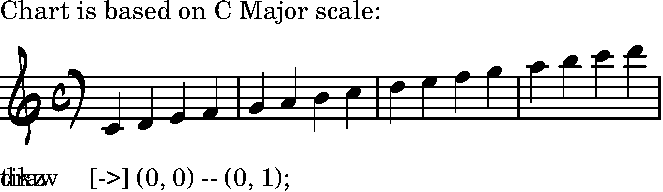
\includegraphics[width=.9\linewidth]{modes-c-major.pdf}
\end{center}
\end{document}
